\chapter{Pruebas $\chi^2$}

\section*{Contenido}
\begin{enumerate}
    \item Introducción
    \item Descripción de la Prueba.
\item $\chi^2$ para una Binomial.
\item $\chi^2$ para una Poisson.
\item $\chi^2$ para una Distribución Uniforme.
\item $\chi^2$ para una Normal.
\item Resumen.
\item Ejercicios.
\end{enumerate}

\section{Introducción}

En el presente capítulo se introducen las pruebas de bondad de ajuste. Se iniciará con las pruebas de bondad de ajuste conocidas como "pruebas de $\chi^2$". Este tipo de pruebas se aplican en estadística a tres problemas que a continuación se detallan. 

Las pruebas de independencia, son un mecanismo estadístico que utiliza proporciones de frecuencias, para determinar si la pertenencia de una variable a un conjunto de categorías es diferente en función de una segunda variable.

Las pruebas de análisis de varianza, o Anova, es una técnica estadística con que se prueba la igualdad de tres o más medias muestrales y que por lo tanto, permite hacer inferencias para determinar si las muestras provienen de poblaciones que tienen la misma media. 

Y por último se utilizan para las pruebas de bondad de ajuste, para determinar si hay una diferencia significativa entre una distribución de frecuencias observadas y una distribución teórica de probabilidad que supuestamente describe la distribución observada.

Se utilizarán las pruebas de bondad de ajuste para dos situaciones. Primero para ver si un generador de números aleatorios produce una buena aproximación de una distribución uniforme. En segundo caso, todo programa de simulación requiere de mecanismos de entrada, de proceso y de salida. Si se tiene un conjunto de observaciones de un modelo real, la prueba de bondad de ajuste nos ayudará a determinar que tipo de distribución se debe utilizar en el modelo de simulación.

\section{Descripción de la Prueba}
Primero, se escriben las hipótesis del problema:

\begin{itemize}
\item[] $H_0$ Esta es una distribución $f(x)$ con sus parámetros
\item[] $H_1$ Esta NO es una distribución $f(x)$ con sus parámetros 
\end{itemize}
\begin{itemize}
\item Se colocan los datos en una tabla de frecuencias, si la distribución es discreta, se cuentan las repeticiones de los números, si la distribución es continua, se suele utilizar $\sqrt{n}$ como el número de intervalos (y se discretizan).

\item Para cada intervalo se coloca la frecuencia observada $fo$
\item  Se debe calcular la probabilidad esperada de la distribución $pe$.
\item Se obtiene la frecuencia esperada $fe$ al convertir $pe$ en frecuencia ($pe\times n$).
\item Se calcula el valor de $\chi²_0$

\item El valor de $\chi²_0$ se comparará con el valor límite de la tabla de $\chi^2$, para ello se requiere un valor $\alpha$ de rechazo o bien un valor de $1-\alpha$ de confiabilidad. Si $\chi^2 \leq \chi^2_{\alpha,gl}$ (siendo $gl$ grados de libertad), se acepta la hipótesis nula de que los números corresponden a una distribución.
\end{itemize}

\section{$\chi^2$ para una Binomial.}

Para un trabajo se han entrevistado a 100 personas. Cada uno de los aspirantes fue entrevistado por 3 ejecutivos. Cada ejecutivo expresó una opinión positiva o negativa de los aspirantes. Se conoce que este tipo de fenómeno se puede describir mediante una distribución binomial.

A continuación se presenta una tabla con el número de opiniones positivas que recibió cada uno de los 100 aspirantes por parte de los tres evaluadores.

\begin{verbatim}

-----------------
x      Frecuencia
       Observada
-----------------
0          18
1          47
2          24
3          11
-----------------
Total     100
-----------------
\end{verbatim}


Si se grafican estas frecuencias observadas se obtiene el siguiente resultado.

\begin{center}
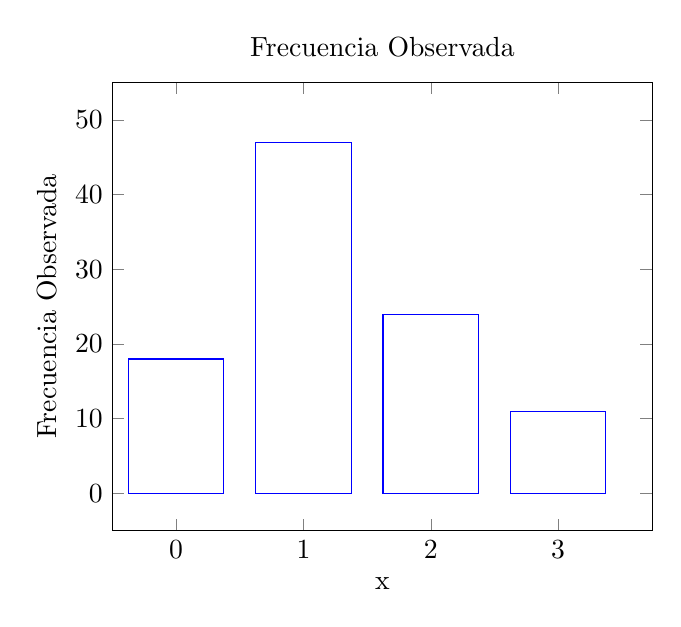
\begin{tikzpicture}
    \begin{axis}[
        title={Frecuencia Observada},
        xlabel={x},
        ylabel={Frecuencia Observada},
        xtick={0,1,2,3},
        ytick={0,10,20,30,40,50},
        grid=both,
        ymin=0, ymax=50,
        xmin=-0.01, xmax=3.25,
        bar width=0.75,
        ymajorgrids=false,
        xmajorgrids=false,
        enlarge x limits=0.15,
        enlarge y limits=0.1,
        ]
        \addplot[ybar, color=blue] 
        coordinates {(0,18) (1,47) (2,24) (3,11)};
    \end{axis}
\end{tikzpicture}
\end{center}

La distribución binomial se representa mediante la fórmula:

$$P(x) = \binom{n}{x} p^x (1-p)^{n-x} \text{    }\forall x \in \{0,1,2,\dots, n\}$$

Cuya esperanza es:
$$E(x) = n\times p$$

Y cuya varianza es:
$$V(x) = n\times p \times (1-p)$$

Como con toda distribución binomial se deben calcular los parámetros de $n$ y $p$. En este caso es evidente por los intervalos que $n = 3$. Sin embargo para calcular el valor de $p$ debemos recurrir al siguiente cálculo:

$$E(x) = \Sigma x \times P(x)$$
$$E(x) = 0 \times \frac{18}{100} + 1 \times \frac{47}{100} + 2 \times \frac{24}{100}+ 3\times \frac{11}{100}$$

$$E(x) = (0 * 0.18) + (1 * 0.47) + (2 * 0.24) + (3 * 0.11)$$

$$E(x) = 1.28$$

Luego se tiene que:

$$E(x) = n * p$$

Despejando la ecuación:
$$1.28 = 3 * p$$
$$p = \frac{1,28}{3}$$
Redondeando a 4 decimales:
$$p = 0.4267$$

Por lo que se generarán las hipótesis usuales y se utilizará un nivel de confianza del $0.95$. O de manera equivalente un valor de $\alpha=0.05$.

\begin{itemize}
\item[] \textbf{$H_0$}: Esta es una distribución binomial 
    con parámetros n=3 y p=0.4267

\item[] \textbf{$H_1$}:: La anterior no es una buena descripción de la distribución

\end{itemize}

Primero debemos proceder a construir las frecuencias esperadas de la distribución, de acuerdo con los supuestos de $H_0$ se tiene que la distribución tiene el siguiente comportamiento.

$$P(x) = \binom{3}{x} 1,4267^x (1-0,4267)^{3-x} \text{    }\forall x \in \{0,1,2,3\}$$

$$P(x) = \binom{3}{x} 1,4267^x (0,5733)^{3-x} \text{    }\forall x \in \{0,1,2,3\}$$

Por lo tanto (redondeando a 4 decimales de precisión):

$$P(0) = \binom{3}{0} 1,4267^0 (0,5733)^{3} = 0.1884 $$
$$P(1) = \binom{3}{1} 1,4267^1 (0,5733)^{3-1} =  0.4207 $$
$$P(2) = \binom{3}{2} 1,4267^2 (0,5733)^{3-2} =  0.3131 $$
$$P(3) = \binom{3}{3} 1,4267^3 (0,5733)^{3-3} = 0.0777$$

Las anteriores constituyen las probabilidades de la distribución, pero debemos obtener las frecuencias esperadas.

\begin{verbatim}

---------------------------------
x   p(x)       p(x) * 100 = fe(x)
---------------------------------
0   0.1884   0.1884 * 100 = 18.84
1   0.4207   0.4207 * 100 = 42.07
2   0.3131   0.3131 * 100 = 31.31
3   0.0777   0.0777 * 100 =  7.77
---------------------------------
\end{verbatim}


Con lo cual se obtiene la siguiente tabla:
\begin{verbatim}
-------------------
x       fo     fe
-------------------
1       18    18.84
2       47    42.07
3       24    31.31
4       11     7.77
-------------------
Total  100   100.00
-------------------
    
\end{verbatim}



Y procedemos a calcular el valor de $\chi^2$:
\begin{verbatim}
-------------------------------------------------
                                     (fo-fe)^2
x   fo    fe    (fo-fe)  (fo-fe)^2   ---------
                                        fe
-------------------------------------------------
0   18   18.84   -0.84    0.7056     0.0375
1   47   42.07    4.93   24.3049     0.5777
2   24   31.31   -7.31   53.4361     1.7067
3   11    7.77    3.23   10.4329     1.3427
-------------------------------------------------
                                                2
                                              \/
                                     3.6646 = /\
                                                0
-------------------------------------------------
    
\end{verbatim}



Para realizar la prueba se utilizará un nivel de confianza de $0.95$ o lo que es equivalente un valor de rechazo $\alpha = 0.05$. Para la determinación de los grados de libertad se deben poner nuevas restricciones. Primero como hay 4 clases, se deben tomar $4-1 = 3$ grados de libertad. Pero como además calculamos el valor de $p$, se debe restar un grado de libertad más es decir $3-1 = 2$.

La regla general es la siguiente, primero se emplea la regla de restar uno al número de clases, $k-1$, y luego se resta un grado de libertad adicional por cada parámetro de población que tenga que ser estimado de los datos de la muestra.  

$$\chi^2_{0.05,2} = 5.9915$$

Al utilizar en la tabla de $\chi^2$, se busca bajo la columna de $0.05$ en la cola derecha de la distribución con 2 grados de libertad y se encuentra el valor de rechazo de $5.9915$. Cómo $3.6646 < 5.9915$ se acepta $H_0$ y se debe tomar como verdadera dicha hipótesis .

\begin{center}
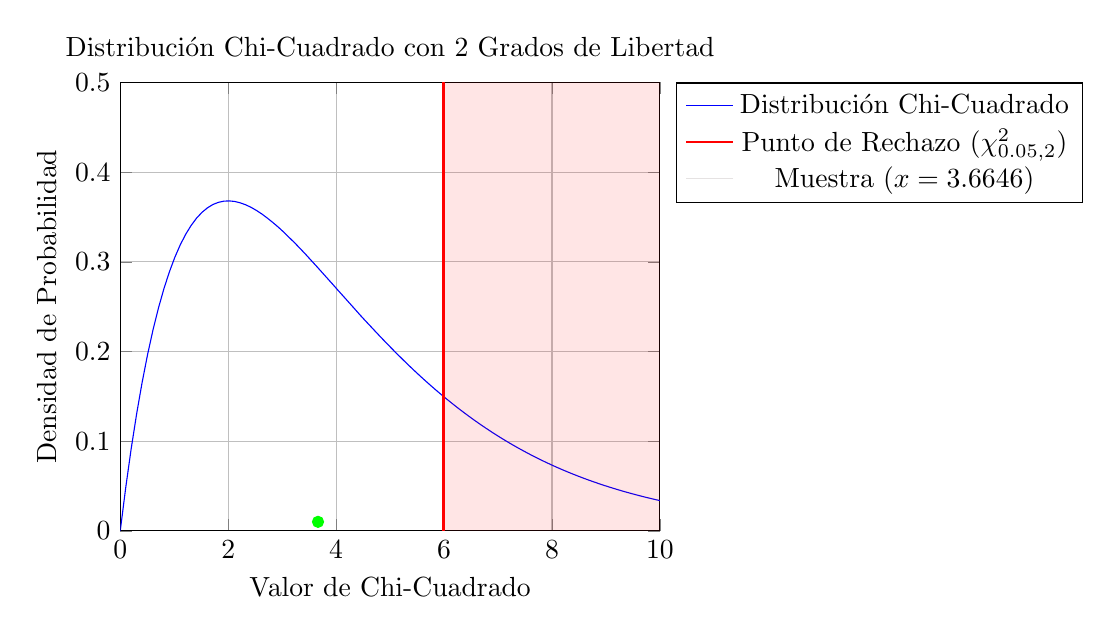
\begin{tikzpicture}
    \begin{axis}[
        title={Distribución Chi-Cuadrado con 2 Grados de Libertad},
        xlabel={Valor de Chi-Cuadrado},
        ylabel={Densidad de Probabilidad},
        xmin=0, xmax=10,
        ymin=0, ymax=0.5,
        grid=both,
        domain=0:10,
        samples=100,
        legend pos=outer north east,
    ]
        % Gráfica de la distribución chi-cuadrado
       \addplot[blue] {(1/2) * x * exp(-x/2)};
        \addlegendentry{Distribución Chi-Cuadrado}

        % Línea vertical para el punto de rechazo
        \addplot[red, thick] coordinates {(5.991, 0) (5.991, 0.5)};
        \addlegendentry{Punto de Rechazo ($\chi^2_{0.05, 2}$)}

        % Marcar el área de rechazo
        \addplot[fill=red, opacity=0.1] 
        coordinates {(5.991, 0) (10, 0) (10, 0.5) (5.991, 0.5)};

        % Punto en x = 3.6646        
        \addplot[mark=*, only marks, mark options={color=green, fill=green}] coordinates {(3.6646, 0.01)};        
        \addlegendentry{Muestra ($x = 3.6646$)}
    \end{axis}
\end{tikzpicture}
\end{center}


\begin{verbatim}




4. $\chi^2$ para una Poisson.
================================

En un hospital de la capital se han recolectado datos del número de pacientes que llega cada hora. Este tipo de fenómeno suele representarse mediante una distribución Poisson. A continuación se presenta una tabla con las frecuencias observadas:

-----------------
x      Frecuencia
       Observada
-----------------
0          25
1          55
2          65
3          35
4          20
5          10
-----------------
Total     210
-----------------



Las frecuencias observadas se pueden representar mediante el siguiente gráfico.



70|
  |      __
60|     |  |
  |   __|  |
50|  |  |  |
  |  |  |  |
40|  |  |  |
  |  |  |  |__
30|  |  |  |  |
  |__|  |  |  |
20|  |  |  |  |__
  |  |  |  |  |  |
10|  |  |  |  |  |__
  |  |  |  |  |  |  |
 0|__|__|__|__|__|__|___
    0  1  2  3  4  5



La distribución Poisson tiene las siguientes características:


       L^x * e^(-L)
p(x) = ------------        para x = 0,1,2,3,...
           x!


                    \
          \ x     - /\
          /\  *  e
p(x)  =  --------------     para x = 0,1,2,3,...
              x!


         \
E(x)  =  /\


         \
V(x)  =  /\



La distribución Poisson tiene como parámetro el valor de lambda. A continuación se procede a calcular este valor.

         __
         \
E(x)  =  /_ x * p(x)



               /     25  \     /     55  \     /      65 \ 
E(x)  =       (  0 * ---  ) + (  1 * ---  ) + (  2 * ---  )
               \     210 /     \     210 /     \     210 / 


               /      35 \     /      20 \       /      10 \ 
          +   (  3 * ---  ) + (  4 * ---  )   + (  5 * ---  )
               \     210 /     \     210 /       \     210 / 

                                                      

          1     /                                         \ 
E(x)  =  --- * (  0*25 + 1*55 + 2*65 + 3*35 + 4*20 + 5*10  )
         210    \                                         / 


               
          1     /                                        \
E(x)  =  --- * (  0   +  55  +  130 +  105 +  80  +  50   )
         210    \                                        /



          1     /     \
E(x)  =  --- * (  420  )
         210    \     /



         420
E(x) =  ----
         210


E(x) =  2



Para la prueba de hipótesis se va a utilizar un valor de lambda de 2. Se generarán las hipótesis usuales y se utilizará un nivel de confianza del 95%.


H0: Esta es una distribución poisson
    con parámetros de lambda = 2


H1: La anterior no es una buena descripción
    de la distribución



Para calcular las frecuencias esperadas de la distribución se utilizan los parámetros encontrados. 


          / 2^x * e^(-2) \
p(x)  =  (  ------------  )   para x = 0,1,2,3,...
          \     x!       /



          / 2^0 * e^(-2) \     /        \
p(0)  =  (  ------------  ) = (  e^(-2)  )  =  0.1353
          \     0!       /     \        /



          / 2^1 * e^(-2) \     /            \ 
p(1)  =  (  ------------  ) = (  2 * e^(-2)  ) =  0.2707
          \     1!       /     \            / 




          / 2^2 * e^(-2) \     / 4 * e^(-2) \     /            \ 
p(2)  =  (  ------------  ) = (  ----------  ) = (  2 * e^(-2)  )  =  0.2707
          \     2!       /     \   2        /     \            / 




          / 2^3 * e^(-2) \     / 8 * e^(-2) \     /  4           \ 
p(3)  =  (  ------------  ) = (  ----------  ) = (  --- * e^(-2)  ) =  0.1804
          \     3!       /     \   6        /     \  3           / 




          / 2^4 * e^(-2) \     / 16 * e^(-2) \     /  2           \ 
p(4)  =  (  ------------  ) = (  -----------  ) = (  --- * e^(-2)  ) =  0.0902
          \     4!       /     \   24        /     \  3           / 



          / 2^5 * e^(-2) \     / 32 * e^(-2) \     /  4           \ 
p(5)  =  (  ------------  ) = (  -----------  ) = (  --- * e^(-2)  ) =  0.0361
          \     5!       /     \   120       /     \  5           / 







Las anteriores constituyen las probabilidades de la distribución, pero debemos convertirlas en frecuencias esperadas.


-----------------------------------
x   p(x)       p(x) * 210 = fe(x)
-----------------------------------
0   0.1353   0.1353 * 210 = 28.4130
1   0.2707   0.2707 * 210 = 56.8470
2   0.2707   0.2707 * 210 = 56.8470
3   0.1840   0.1804 * 210 = 37.8840
4   0.0902   0.0902 * 210 = 18.9420
5   0.0361   0.0361 * 210 =  7.5810
-----------------------------------



De esta forma tenemos los valores de las frecuencias observadas y las frecuencias esperadas.

----------------------
x        fo    fe
----------------------
0        25    28.4130
1        55    56.8470
2        65    56.8470 
3        35    37.8840
4        20    18.9420
5        10     7.5810
----------------------
Total   210   206.5140
----------------------



Procedemos a calcular el valor de $\chi^2$:

-----------------------------------------------------
                                         (fo-fe)^2
n   fo     fe       (fo-fe)   (fo-fe)^2  ---------
                                            fe
-----------------------------------------------------
0   25   28.4130   -3.4130   11.6490     0.4100
1   55   56.8470   -1.8470    3.4110     0.0600
2   65   56.8470    8.1530   66.4710     1.1690
3   35   37.8840   -2.8840    8.3170     0.2200
4   20   18.9420    1.0580    1.1190     0.0590 
5   10    7.5810    2.4190    5.8520     0.7720
-----------------------------------------------------
                                                    2
                                                  \/
                                         2.6906 = /\
                                                    0
-----------------------------------------------------



Para realizar la prueba se utiliza el nivel de confianza de 0.95 o lo que es equivalente un valor de rechazo $\alpha = 0.05$. Para calcular los grados de libertad como se tienen 6 intervalos inicialmente se resta un grado, 6-1 = 5. Posteriormente como se calculó el valor de lambda restamos un grado más 6-2 = 4.


  2
\/
/\(0.05,4) = 9.4877


Al utilizar la tabla de $\chi^2$, se busca bajo la columna de 0.05 en la cola derecha con 4 grados de libertad y se encuentra el valor de rechazo de 9.4877. Cómo 2.6906 < 9,4877 se acepta H0.



|
|                   
|                 . ' .
|               .       .
|             .           .
|            .              .      |
|           .                 .    |
|          .                     . |
|        .                         | .
|     .                            |      .
|__________________________________|______________________
            |                      |    
           2.6906                 9.4877   




5. $\chi^2$ para una Distribución Uniforme.
==============================================

Se han generado 100 números aleatorios en el intervalo de [0,1[ y se han distribuido en cinco intervalos pues se desean utilizar este generador para generar números uniformes enteros entre [1,5]. Estos valores suelen llamarse la frecuencia observada.

------------------------------
No.    Intervalos   Frecuencia
                     Observada
------------------------------
1      [0.00,0.20[      21
2      [0.20,0.40[      22
3      [0.40,0.60[      19
4      [0.60,0.80[      23
5      [0.80,1.00[      15
------------------------------
Total                  100
------------------------------



De inmediato es visible que el comportamiento de este generador no es del todo simétrico.



23|             __
22|       __   |  |
21|    __|  |  |  |
20|   |  |  |  |  |
19|   |  |  |__|  |
18|   |  |  |  |  |
17|   |  |  |  |  |
16|   |  |  |  |  |
15|   |  |  |  |  |__
  =   |  |  |  |  |  |
 0|___|__|__|__|__|__|___
       1  2  3  4  5



Y trataremos de equiparar esta frecuencia observada con la frecuencia esperada dada por el gráfico siguiente, con una observación esperada de 20 en cada intervalo.



23|
22|
21|
20|    __ __ __ __ __
19|   |  |  |  |  |  |
18|   |  |  |  |  |  |
17|   |  |  |  |  |  |
16|   |  |  |  |  |  |
15|   |  |  |  |  |  |
  =   |  |  |  |  |  |
 0|___|__|__|__|__|__|___
       1  2  3  4  5



La distribución uniforme se suele presentar en los libros de texto de manera continua, mediante la siguiente expresión:


          /    1
         /   -----   si a <= x <= b
        /    b - a
f(x) = (
        \
         \
          \  0   en otro caso




En nuestro caso particular, con a=0 y b=1, esta distribución se puede reescribir como:
 
        /   1   si 0 <= x <= 1   
f(x) = (
        \   0 en cualquier otro caso



Representada gráficamente como:


    f(x)
      |
      |
      |
    1 |..............
      |             .
      |             .
      |             .
      |             .
      |             .
______|_____________.________ x
      0             1




Por lo que la distribución acumulada está dada por:


          _
         | )x     
F(x) =   |     1  dt   
       (_|  0


 
       |      |x
F(x) = |  t   |
       |      |0



F(x) =  x - 0
      

         
F(x) =  x
        



Por lo que la distribución acumulada de probabilidad se expresa mediante la fórmula:


          /  0    si x <= 0
         /    
F(x) =  (    x    si 0 <= x <= 1
         \    
          \  1    si x >= 1





Gráficamente se representan como:


    F(x)
      |
      |
      |
    1 |            .  .  .  .
      |          .
      |        .
      |      .
      |    .
      |  .
. . . ._____________________
                 1




Con esta distribución se pueden calcular las probabilidades acumuladas para cada uno de los intervalos:


p(0.00 <= x < 0.20) = F(0.20) - F(0.00)
                     = 0.20 - 0
                     = 0.20

                  
p(0.20 <= x < 0.40) = F(0.40) - F(0.20)                  
                    = 0.40 - 0.20
                    = 0.20

                    
p(0.40 <= x < 0.60) = F(0.60) - F(0.40)
                    = 0.60 - 0.40
                    = 0.20

                    
p(0.60 <= x < 0.80) = F(0.80) - F(0.60)
                    = 0.80 - 0.60
                    = 0.20

                    
p(0.80 <= x < 1.00) = F(1.00) - F(0.80)
                    = 1.00 - 0.80
                    = 0.20
                    
                    
Para obtener la frecuencia esperada se deben convertir las probabilidades esperadas en frecuencias.


-----------------------------------
x   p(x)       p(x) * 210 = fe(x)
-----------------------------------
0   0.2000   0.2000 * 100 = 20.0000
1   0.2000   0.2000 * 100 = 20.0000
2   0.2000   0.2000 * 100 = 20.0000
3   0.2000   0.2000 * 100 = 20.0000
4   0.2000   0.2000 * 100 = 20.0000
5   0.2000   0.2000 * 100 = 20.0000
-----------------------------------
                   
                    

Asimismo para llevar a cabo el experimento estadístico se formulan dos hipótesis, se tratará de probar estas hipótesis con una confianza estadística de 0.95.


H0: Esta es una distribución uniforme

H1: Esta NO es una distribución uniforme

 
Si esta fuera efectivamente una distribución uniforme perfecta entonces se esperaría que quedaran 20 números dentro de cada intervalo. Esta se conoce como la frecuencia esperada. A continuación se muestra una tabla con estos datos.


----------------------------
No.  Intervalos    fo   fe
----------------------------
1    [0.00,0.20[   21   20
2    [0.20,0.40[   22   20
3    [0.40,0.60[   19   20
4    [0.60,0.80[   23   20
5    [0.80,1.00[   15   20
----------------------------
Total             100  100
----------------------------


Para la prueba estadística se debe calcular un valor denominado $\chi^2$ subcero, que es la distribución que pronostica el comportamiento de estos números. Para ello se realiza el siguiente cálculo:

------------------------------------------------------------
                                                  (fo-fe)^2
No.  Intervalos     fo   fe   (fo-fe)  (fo-fe)^2   --------
                                                     fe
------------------------------------------------------------
1    [0.00,0.20[    21   20      1        1        0.05
2    [0.20,0.40[    22   20      2        4        0.20
3    [0.40,0.60[    19   20     -1        1        0.05
4    [0.60,0.80[    23   20      3        9        0.45
5    [0.80,1.00[    15   20     -5       25        1.25
------------------------------------------------------------
                                                            2
                                                          \/
                                                   2.00 = /\
                                                            0
_____________________________________________________________



Para realizar la prueba se utilizará un nivel de confianza de 0.95 o lo que es equivalente un valor de rechazo llamado $\alpha = 0.05$. Para estimar los grados de libertad nos vemos obligados a poner más restricciones. Si se tienen k clases, 5 en nuestro ejemplo, se tienen que utilizar k-1 grados de libertad, o sea 5-1 = 4 grados de libertad, una vez que se han puesto valores de las k-1 clases el valor de la clase restante está determinado, de ahí la pérdida de un grado de libertad.

Al buscar en la tabla de $\chi^2$ se busca debajo de la columna que indica 0.05 en la zona derecha de la distribución, lo cual da un valor de 9.4877.


  2
\/
/\ (0.05,4) = 9.4877
  

Como el valor calculado de $\chi^2$ es de 2, este se encuentra a la izquierda del valor de rechazo de 9.4877, es decir 2 < 9.4877, por lo tanto se acepta la hipótesis H0, que dice esta es una distribución uniforme con una confianza del 95%.



|
|
|                 . ' .
|               .       .
|             .           .
|            .              .      |
|           .                 .    |
|          .                     . |
|        .                         | .
|     .                            |      .
|__________________________________|______________________
             |                     |  
             2                    9.4877




6. $\chi^2$ para una Normal.
===============================

Una entidad bancaria desea conservar una cierta cantidad de dinero en efectivo en su bóveda. La cantidad de dinero no debe ser tan poca que el banco no pueda dar dinero, ni tan grande que resulte tentador para los ladrones. Por lo tanto se tiene la idea que la distribución del dinero es normal. Para tal efecto se ha reunido la siguiente información.


---------------------------
Depósitos        Frecuencia
                 Observada
---------------------------
[   0 , 1000 [      20
[1000 , 2000 [      65
[2000 , 3000 [      25
---------------------------
Total              110
---------------------------



Las frecuencias observadas se pueden representar mediante el siguiente gráfico.


  |
60|          ______
  |         |      |
45|         |      |
  |         |      |
30|         |      |______
  |   ______|      |      |
15|  |      |      |      |
  |  |      |      |      |
 0|__|______|______|______|____
      [   0, [1000, [2000,
       1000[  2000[  3000[




La distribución normal se representa mediante la fórmula:



         e^ ((-1/2)*((x-u)/o)^2)
f(x)  =  -----------------------
             o * sqrt(2*pi)



                                  2
               / -1 \   / x - u  \
              (  --  )*(  ------  )
            _  \  2 /   \   o    /
           |_|
           |_
f(x)  =   -------------------------     -oo <= x <= +oo
                         _______
                        /    __
                o  *  \/ 2 * ||



E(x)  =  u


V(x)  =  o^2


de(x) =  o




En el caso de datos agrupados calcular la media y la desviación estándar puede ocasionar problemas o desviaciones. Como se tienen intervalos, para el cálculo de la media, la variancia y la desviación estándar se utiliza el punto medio de cada clase, denotado por x(m).

         __
         \
E(x)  =  /_  x(m) * p(x)



         /        20 \     /         65 \     /         25 \
E(x)  = (  500 * ---  ) + (  1500 * ---  ) + (  2500 * ---  )
         \       110 /     \        110 /     \       110  /



E(x)  =  1545.4545




Para el cálculo de la varianza se utiliza de igual forma el punto medio de cada clase.

         __
         \            _  
V(x)  =  /_  ( x(m) - x )^2  *  p(x)



V(x) =  ( 500 - 1545.45)^2  *  (20/100)

     +  (1500 - 1545.45)^2  *  (65/110)

     +  (2500 - 1545.45)^2  *  (25/110)


V(x)  =  406894.6455


de(x) =  sqrt(406894.6455)


de(x) =     637.8829  



Para la prueba de hipótesis se van a utilizar los valores de la media de 1500 y de la desviación estándar de 600 que se supondrá fueron tomados de la población original. Por lo tanto no se utilizarán los valores calculados para esta distribución normal, por lo que no se restarán grados de libertad adicionales. Es necesario hacer esto ya que se cuentan con muy pocos intervalos. Se generarán las hipótesis usuales y se utilizará un nivel de confianza del 80%.


H0: Esta es una distribución normal
    con media = 1500 y una desviación estándar de 600

H1: La anterior no es una buena descripción
    de la distribución



El cálculo de las probabilidades esperadas se genera utilizando las tablas normales de los apéndices. Observe que estas tablas normales están acumuladas de izquierda a derecha.


P( 0 <= x <= 1000) =  P(x<=1000) - P(x<=0)


                        /      1000-1500 \      /      0 -1500   \
P( 0 <= x <= 1000) =  P(  x <= ---------  ) - P(  x <= ---------  )
                        \        600     /      \        600     /


P( 0 <= x <= 1000) =  P( x <= -0.83 ) - P( x <= -2.50 )


P( 0 <= x <= 1000) =  0.2033 - 0.0062


P(   0 <= x <= 1000) = 0.1971




P(1000 <= x <= 2000) =  P(x<=2000) - P(x<=1000)


                          /      2000-1500 \      /      1000-1500 \
P(1000 <= x <= 2000) =  P(  x <= ---------  ) - P(  x <= ---------  )
                          \        600     /      \        600     /


P(1000 <= x <= 2000) =  P( x <=  0.83 ) - P( x <= -0.83 )


P(1000 <= x <= 2000) =  0.7967 - 0.2033


P(1000 <= x <= 2000) = 0.5934




P(2000 <= x <= 3000) =  P(x<=3000) - P(x<=2000)


                          /      3000-1500 \      /      2000-1500 \ 
P(2000 <= x <= 3000) =  P(  x <= ---------  ) - P(  x <= ---------  )
                          \        600     /      \        600     / 


P(2000 <= x <= 3000) =  P( x <=  2.50 ) - P( x <=  0.83 )


P(2000 <= x <= 3000) =  0.9938 - 0.7967


P(2000 <= x <= 3000) = 0.1971



A continuación se muestra la tabla en donde se convierten las probabilidades en las frecuencias esperadas correspondientes.


----------------------------------------------
Intervalo      p(x)       p(x) * 110 = fe(x)
----------------------------------------------
[   0 , 1000[  0.1971   0.1971 * 110 = 21.6810
[1000 , 2000[  0.5934   0.5934 * 110 = 65.2740
[2000 , 3000[  0.1971   0.1971 * 110 = 21.6810
----------------------------------------------



Con los datos anteriores se calcula el estadístico de $\chi^2$ para la prueba de bondad de ajuste.


--------------------------------------------------------------
                                                 (fo-fe)^2
Intervalo       fo   fe       fo-fe   (fo-fe)^2  ---------
                                                     fe
--------------------------------------------------------------
[   0 , 1000[   20  21.6810  -1.6810   2.8258    0.1303
[1000 , 2000[   65  65.2740  -0.2740   0.0751    0.0012
[2000 , 3000[   25  21.6810   3.3190  11.0158    0.5081
--------------------------------------------------------------
                                                             2
                                                           \/
                                                 0.6396 =  /\
                                                             0
--------------------------------------------------------------


Para realizar la prueba se utilizará un nivel de confianza de 0.90 o lo que es equivalente un valor de rechazo alfa = 0.10. Para calcular los grados de libertad como se tienen 3 intervalos inicialmente restamos uno, 3-1 = 2. Posteriormente si se hubieran utilizado los valores calculados de la media y la desviación estándar se deberían restar dos grados adicionales. Esto dejaría los grados de libertad en 0, lo que indica que el número de intervalos es muy pequeño. Por esta razón se utilizaron los parámetros provenientes de la población original y solamente se resta un grado de libertad.


  2
\/
/\ (0.10,2) = 4.6052



Al utilizar la tabla de $\chi^2$, se debe buscar bajo la columna de 0.10 en la cola derecha con 2 grados de libertad y encontramos el valor de rechazo de 4.6052. Cómo 0.6396 < 4.6052 se acepta H0.



|
|
|                 . ' .
|               .       .
|             .           .
|            .              .      |
|           .                 .    |
|          .                     . |
|        .                         | .
|     .                            |      .
|__________________________________|______________________
            |                      |    
           0.6396                 4.6052   





7. Resumen.
===========

Para determinar el tipo de distribución, además de tomar en cuenta las frecuencias observadas se debe conocer qué tipo de fenómeno produjo estas observaciones.

Las pruebas de $\chi^2$ nos permiten dado un conjunto de datos preguntarnos que distribución es la más apropiada para representarlos. Esta prueba nos permite saber si existe una diferencia significativa entre una distribución observada y una distribución teórica. De esta forma estamos en condiciones de determinar la bondad de ajuste de una distribución teórica.  En otras palabras podemos precisar hasta que punto encaja la distribución en los datos que hemos observado. Se puede por lo tanto concluir si los datos observados constituyen una muestra extraída de la distribución teórica.

Dentro de la prueba es importante determinar el número de grados de libertad de la misma. Para ello se utiliza la fórmula de (n - 1 - k), donde "k" representa el número de parámetros que se extrajeron de los datos.



 
8. Ejercicios.
==============



() Ejercicio 1

Se lanzó un dado 600 veces, con los siguientes resultados.

---------------------
Valor    Frecuencia
Dado     Observada
---------------------
  1          89
  2         113
  3          98
  4         104
  5         117
  6          79
---------------------
Total       600
---------------------


Determine si el dado está balanceado, es decir, se trata de un dado legal. Para ello utilice un nivel de alfa de 0.05




() Ejercicio 2

La teoría de Mendell establece que los frijoles se pueden clasificar en cuatro categorías. Categoría I es  redondo y amarillo, la categoría II es rugoso y amarillo, la categoría III es redondo y verde y la categoría IV es rugoso y verde. Asimismo la distribución de los frijoles en estas categorías debe ser de la forma 9,3,3,1 para cada categoría respectivamente. Se tomaron 100 frijoles al azar y se encontró la siguiente distribución:

----------------------
Categoría   Frecuencia
            Observada
----------------------
  I           56
  II          19
  III         17
  IV           8
----------------------
Total        100
----------------------


Haga una prueba de $\chi^2$ para determinar si estos datos son congruentes con el modelo propuesto. Utilice un valor de alfa de 0.05



() Ejercicio 3

A la empresa LL tiene 5 clientes que la visitan por día. Se cree que las ventas realizadas por día se pueden describir mediante una distribución binomial, con una probabilidad de 0.40 de lograr la venta. A continuación se presentan los datos obtenidos.

---------------------
Ventas    Frecuencia
          Observada
---------------------
  0          10
  1          41
  2          60
  3          20
  4           6
  5           3
---------------------


a. Es el valor de 0.40 adecuado para los datos obtenidos.
b. Realice una prueba de bondad de ajuste con 0.40 y un nivel de alfa de 0.05.
c. Realice una prueba de bondad de ajuste con el valor que encontró usted para la distribución en el primer punto y alfa de 0.05



() Ejercicio 4

A continuación se presentan un conjunto de datos que se cree pertenecen a una distribución de Poisson. Con un nivel de alfa de 0.10 compruebe si es verdadero o no.

----------------------
Llegadas   Frecuencia
por Hora   Observada
----------------------
    0         10
    1         15
    2         26
    3         31
    4         15
    5          3
----------------------



() Ejercicio 5

La Oficina de Correos desea estudiar el problema de cartas y envíos que llegan en mal estado. Se cree que existe una probabilidad de 0.15 que una carta llegue en mal estado. Para ello se seleccionaron 310 personas y se les enviaron 2 cartas a cada persona. A continuación se dan los datos que se reunieron:

------------------------
Cartas        Frecuencia
Maltratadas   Observada
------------------------
    0         260
    1          40
    2          10
------------------------
Total         310
------------------------


a. ¿Qué tipo de distribución se apega a estos datos?

b. Realice una prueba de bondad de ajuste para establecer si esta distribución corresponde adecuadamente a los datos. Utilice un alfa de 0.10

c. Calcule los parámetros con base en las frecuencias observadas e indique si corresponden a los parámetros mencionados.




() Ejercicio 6

La Junta de Protección Social, encarga de la emisión de lotería, está estudiando la posibilidad de sacar al mercado un nuevo juego. Se estima que en este nuevo juego hay un 5% de ganar un premio de $100, un 10% de probabilidad de ganar un premio de $1, , y un 85% de probabilidad de no ganar nada. Para ver si esta afirmación es correcta se ha tomado una muestra de 1000 tiquetes de lotería del nuevo juego. En esta muestra se obtuvieron, 55 premios de $100, 80 premios de $1 y 865 tiquetes sin ningún premio.

Si se utiliza un nivel de alfa de 0.05 indique si es correcta la suposición de la Junta de cómo están establecidas las probabilidades de este nuevo juego.




() Ejercicio 7

Un jugador profesional de "baseball" participó en 100 juegos. Durante estos juegos obtuvo los siguientes resultados. El jugador sostiene que tiene una probabilidad de 0.4 de batear un hit cuando toma su turno al bate y de 0.60 de no batear. Se han recopilado los siguientes datos.


-------------------------------------
Hits         Número de juegos
Conectados   en que conectó esos hits
-------------------------------------
    0        15
    1        35
    2        30
    3        15
    4         5
-------------------------------------
Total       100
-------------------------------------


a. Identifique el tipo de distribución y obtenga los parámetros que sean necesarios para establecer si la observación del bateador es cierta.

b. Realice una prueba de bondad de ajuste con un nivel de alfa de 0.05 para determinar si estos datos corresponden a la distribución indicada utilizando los parámetros originales del problema.




() Ejercicio 8

Se cuentan con los siguientes datos de ventas:

---------------------------
Intervalos   Frecuencia
             Observada
---------------------------
[60 , 65[      10
[65 , 70[      20
[70 , 75[      40
[75 , 80[      50
[80 , 85[      40
[85 , 90[      40
---------------------------
Total         200
---------------------------


a. Realice una prueba de bondad de ajuste, si se cree que los datos provienen de una distribución normal, con un media de 78 y una desviación estándar de 9. Utilice un valor de alfa de 0.10.

b. Con lo datos que se tienen, se pueden estimar los valores de la media y de la desviación estándar de la distribución. Si o no, justifique su respuesta. En caso de responder afirmativamente proceda a calcular estos parámetros.




() Ejercicio 9

A continuación se presentan un conjunto de frecuencias observadas que provienen de una distribución normal con una media de 3 y una desviación estándar de 0.5

---------------------------
Valor            Frecuencia
                 Observada
---------------------------
] -oo , 2.20[        3
[2.20 , 2.60[       17
[2.60 , 3.00[       33
[3.00 , 3.40[       22
[3.40 , +oo [        5
---------------------------


a. Realice una prueba de bondad de ajuste, utilizando los parámetros de la normal, con un valor de alfa de 0.10.

b. Con lo datos que se tienen, se pueden estimar los valores de la media y de la desviación estándar de la distribución. Si o no, justifique su respuesta. En caso de responder afirmativamente proceda a calcular estos parámetros.



() Ejercicio 10

Un hospital ha estado analizando el peso de su población adulta. Ellos tienen la hipótesis que el peso se distribuye de manera normal con una media de 71 y una desviación estándar de 15. Para probar esto se reunió la siguiente tabla de datos.

-------------------------------------------------
 70   72   69   52   90   55   86   94   58   57
 73   71   87   91   84   95   55   52   66   95
 86   56   58   51   55   90   65   87   50   56
 57   84   64   80   58   55   98   58   82   55
 85   62   78   61   81   92   62   59   88   65
-------------------------------------------------


a. Obtenga la media y la desviación estándar de la muestra y compárela con las propuestas.

b. Haga una prueba de $\chi^2$ para determinar si esta es una distribución normal con los parámetros descritos. Utilice un nivel de alfa de 0.10. Sugerencia para esta prueba utilice 5 intervalos, donde cada uno tenga la misma probabilidad.


\end{verbatim}